%
% fourier.tex -- slide template
%
% (c) 2021 Prof Dr Andreas Müller, OST Ostschweizer Fachhochschule
%
\bgroup
\begin{frame}[t]
\setlength{\abovedisplayskip}{5pt}
\setlength{\belowdisplayskip}{5pt}
\frametitle{Fourier-Transformation}
\vspace{-20pt}
\begin{columns}[t,onlytextwidth]
\begin{column}{0.48\textwidth}
\begin{block}{Aufgabe}
Gegeben: Funktion $f$ auf dem Graphen
\\
\uncover<2->{%
Gesucht: Koeffizienten $\hat{f}$ der Darstellung in der Laplace-Basis}
\end{block}
\uncover<3->{%
\begin{block}{Definition $\chi$-Matrix}
Eigenwerte $0=\lambda_1<\lambda_2\le \dots \le \lambda_n$ von $L$
\vspace{-10pt}
\begin{center}
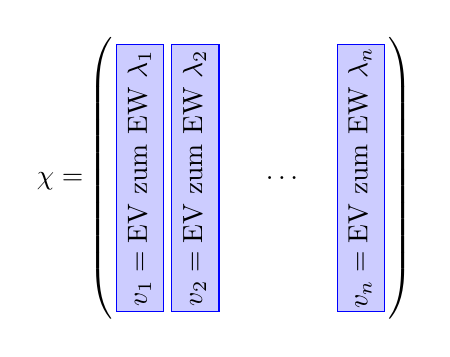
\begin{tikzpicture}
\node at (-1.9,0) [left] {$\chi=\mathstrut$};
\node at (0,0) {$\left(\raisebox{0pt}[1.7cm][1.7cm]{\hspace{3.5cm}}\right)$};

\fill[color=blue!20] (-1.7,-1.7) rectangle (-1.1,1.7);
\draw[color=blue] (-1.7,-1.7) rectangle (-1.1,1.7);
\node at (-1.4,0) [rotate=90] {$v_1=\mathstrut$EV zum EW $\lambda_1$\strut};

\fill[color=blue!20] (-1.0,-1.7) rectangle (-0.4,1.7);
\draw[color=blue] (-1.0,-1.7) rectangle (-0.4,1.7);
\node at (-0.7,0) [rotate=90] {$v_2=\mathstrut$EV zum EW $\lambda_2$\strut};

\fill[color=blue!20] (1.1,-1.7) rectangle (1.7,1.7);
\draw[color=blue] (1.1,-1.7) rectangle (1.7,1.7);
\node at (1.4,0) [rotate=90] {$v_n=\mathstrut$EV zum EW $\lambda_n$\strut};

\node at (0.4,0) {$\dots$};

\end{tikzpicture}
\end{center}
\end{block}}
\end{column}
\begin{column}{0.48\textwidth}
\uncover<4->{%
\begin{block}{Transformation}
$L$ symmetrisch
\\
\uncover<5->{$\Rightarrow$ 
Die Eigenvektoren von $L$ können orthonormiert gewählt werden}
\\
\uncover<6->{$\Rightarrow$ 
Koeffizienten können durch Skalarprodukte ermittelt werden:}
\uncover<7->{%
\[
\hat{f}(k)
=
\hat{f}(\lambda_k)
\uncover<8->{=
\langle v_k, f\rangle
\quad\Rightarrow\quad
\hat{f}}
\uncover<9->{=
\chi^tf}
\]}
\uncover<10->{%
$\chi$ ist die {\em Fourier-Transformation}}
\end{block}}
\uncover<11->{%
\begin{block}{Rücktransformation}
Eigenvektoren orthonormiert
\\
\uncover<12->{$\Rightarrow$
$\chi$ orthogonal}
\uncover<13->{
\[
\chi\chi^t = I
\]}
\end{block}}
\end{column}
\end{columns}
\end{frame}
\egroup
